Esquematico del circuito a implementar:
\begin{figure}[H]
    \centering
    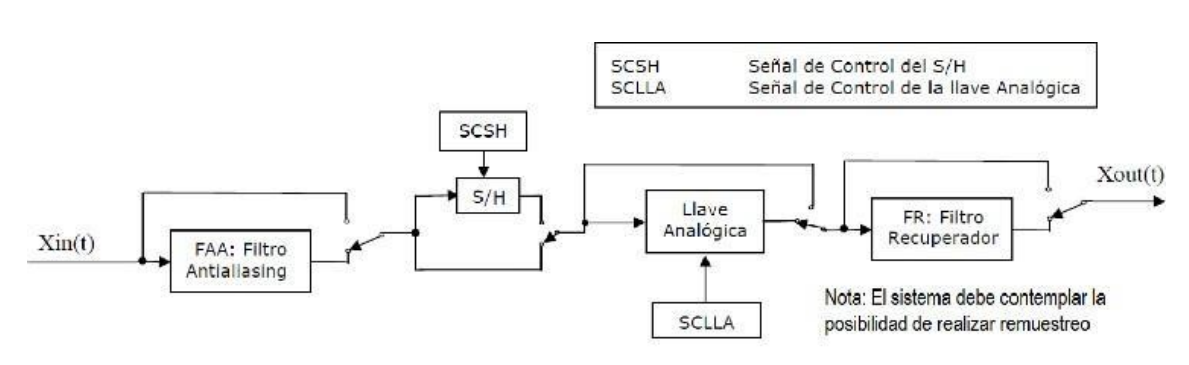
\includegraphics[width=0.8\textwidth]{Imagenes/Circuito_Muestreo.png}
    \caption{Circuito de Muestreo y Retención}
    \label{fig:Circuito_Muestreo}
\end{figure}
Esta implementación del circuito de muestreo y recuperación de la señal analógica nos permite analizar 
los efectos de las distintas etapas del proceso de muestreo y su importancia en el sampleo de la señal.
\subsection{Filtros Pasabajos}
holahola

\subsection{Oscilador}

\subsection{Obtención de Señal Muestreada}

